\documentclass[hyperref=colorlinks]{beamer}
\mode<presentation>
\usetheme{iclpt}
\setbeamertemplate{navigation symbols}{}
\setbeamertemplate{headline}{
\begin{beamercolorbox}[leftskip=.2cm,rightskip=.2cm,topskip=.2cm,ht=1.1cm,dp=0.1cm,wd=\textwidth]{institute in head/foot}
  
\includegraphics[height=1cm]{icl.pdf}
  \hfill
  
\includegraphics[height=1cm]{../Pics/CMS-Color.pdf}
\end{beamercolorbox}
}
\setbeamertemplate{footline}{
\begin{beamercolorbox}[ht=.55cm,dp=0.4cm,wd=\textwidth,leftskip=.3cm]{author in head/foot}%
  \begin{minipage}[c]{5cm}%
    \usebeamerfont{author in head/foot}
    \insertshortauthor 
    \insertshorttitle
    \end{minipage}\hfill%
  \insertframenumber{} / \pageref{lastframe}
  \hfill
  \begin{minipage}{6cm}
    \hfill
  \end{minipage}
\end{beamercolorbox}%
}

\usepackage{color}
\usepackage{tabularx,colortbl}
\usepackage{graphicx}
\usepackage{pdfpages}
\usepackage{feynmp}
\usepackage{tikz}
\usetikzlibrary{calc, shapes, backgrounds,arrows,positioning}
\DeclareGraphicsRule{*}{mps}{*}{}

\title{\vspace{-0.2cm} 40 pb$^{-1}$ Data}
\subtitle{\vspace{-0.7cm}}
\author[]{}%\underline{P. Dunne}} % A.M. Magnan and A. Nikitenko Joao Pela with \\ R. Aggleton, J. Brooke: Bristol \\ C.Asawangtrakuldee, Q.Li: Peking \\ P. Srimanobhas: Chulalongkorn \\ S. Kumar, K. Mazumdar: Mumbai}
\titlegraphic{
  \vspace{-0.7cm}
  %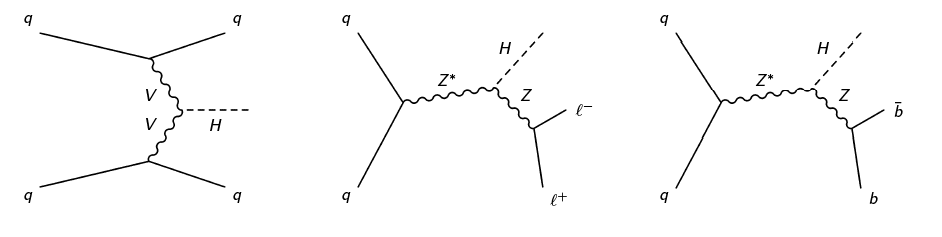
\includegraphics[width=\textwidth]{TalkPics/invcomb021213/feyndiags}
  %% \begin{fmfgraph*}(100,70)
  %%         \fmfleft{i1,i2}
  %%         \fmfright{o1,o2,o3}
  %%         \fmf{fermion}{i1,v1,o1}
  %%         \fmf{fermion}{i2,v2,o3}
  %%         \fmf{phantom,tension=4/5}{v1,v2}
  %%         \fmffreeze
  %%         \fmf{photon,label=$W,,Z$}{v1,v3}
  %%         \fmf{photon,label=$W,,Z$}{v2,v3}
  %%         \fmf{dashes}{v3,o2}
  %%         \fmflabel{$q$}{i1}
  %%         \fmflabel{$q$}{i2}
  %%         \fmflabel{$q$}{o1}
  %%         \fmflabel{$q$}{o3}
  %%         \fmflabel{$H$}{o2}
  %%       \end{fmfgraph*}
}
\date{}
\begin{document}
\begin{fmffile}{higgsexoupdatefeyndiags}
\tikzstyle{every picture}+=[remember picture]

%TITLE PAGE
\section{Title}
\begin{frame}
  \titlepage
  
\end{frame}

\begin{frame}
  \frametitle{Reminder}
  \begin{block}{}
    \begin{itemize}
    \item We now have the full 40 pb$^{-1}$ of MET and SingleMuon PDs processed
    \item Two datasets for each due to first part of PromptReco missing Met Filters
    \item Will show plots of variables used in trigger
    \end{itemize}
    \end{block}
\end{frame}

\begin{frame}
  \frametitle{Trigger variables: pass trigger}
  \begin{block}{}
    \begin{itemize}
    \item Start by requiring only HLT\_DiPFJet40\_DEta3p5\_MJJ600\_PFMETNoMu140\_v
    \end{itemize}
  \end{block}
  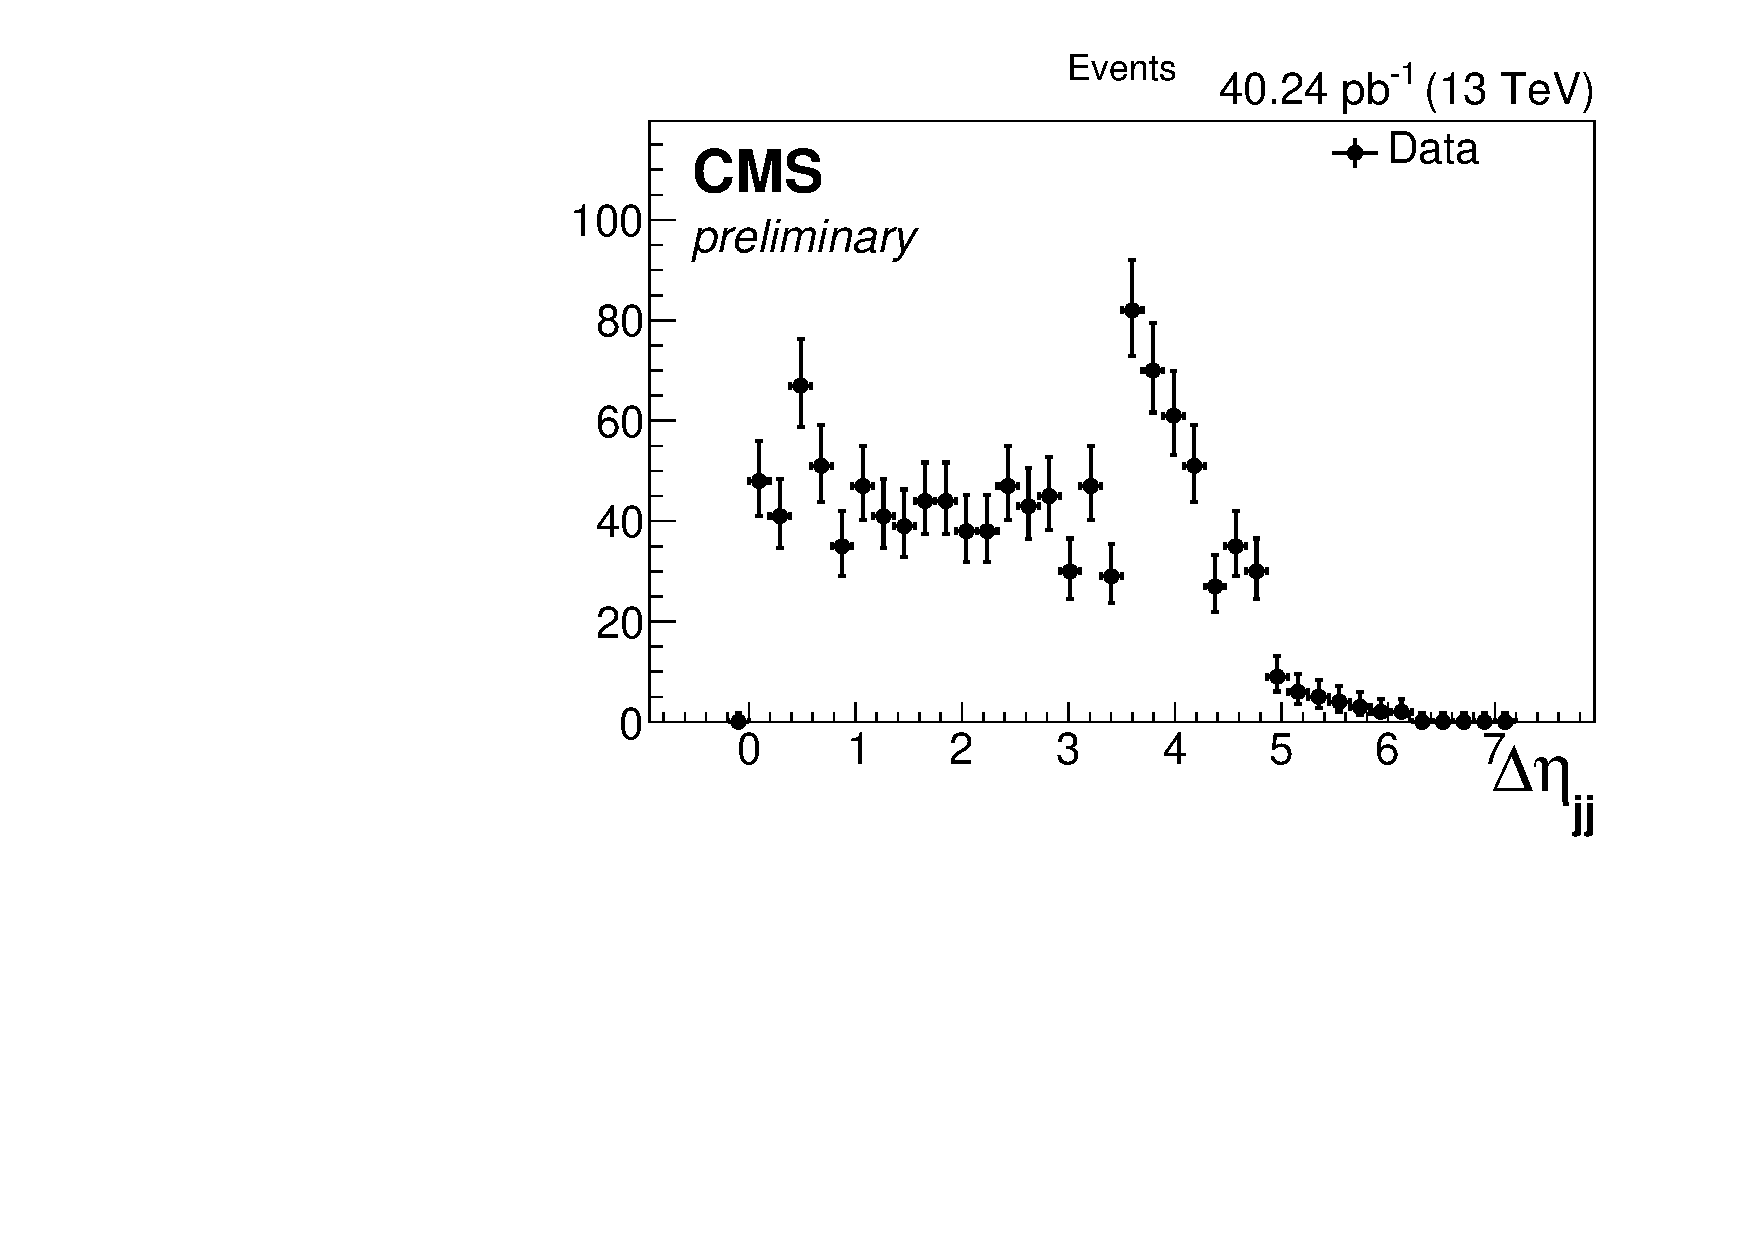
\includegraphics[width=.5\textwidth]{TalkPics/dataplots030815/output/nunu_dijet_deta.pdf}
  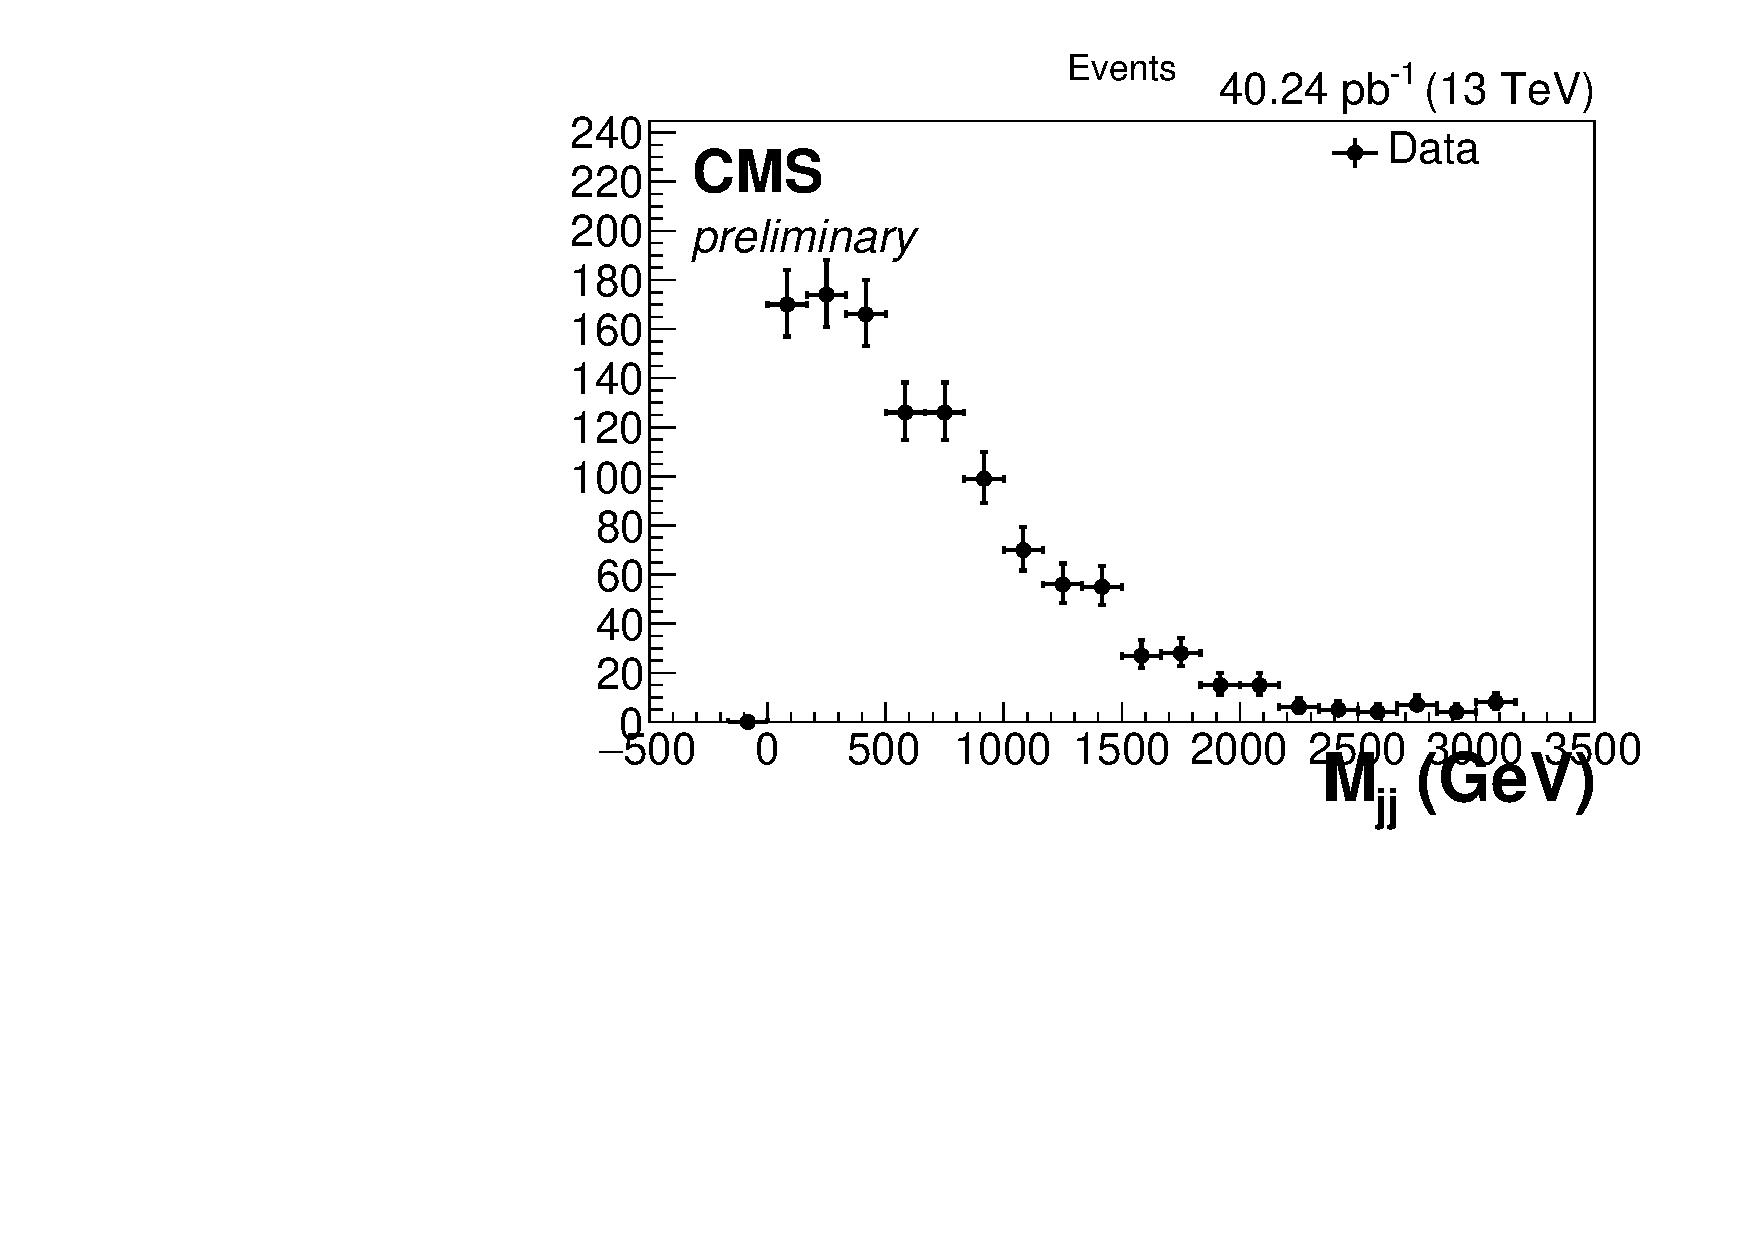
\includegraphics[width=.5\textwidth]{TalkPics/dataplots030815/output/nunu_dijet_M.pdf}
  \begin{block}{}
    \begin{itemize}
    \item Clearly different jet pair offline
    \end{itemize}
  \end{block}
\end{frame}

\begin{frame}
  \frametitle{Trigger variables: pass trigger}
  \begin{block}{}
    \begin{itemize}
    \item Start by requiring only HLT\_DiPFJet40\_DEta3p5\_MJJ600\_PFMETNoMu140\_v
    \end{itemize}
  \end{block}
  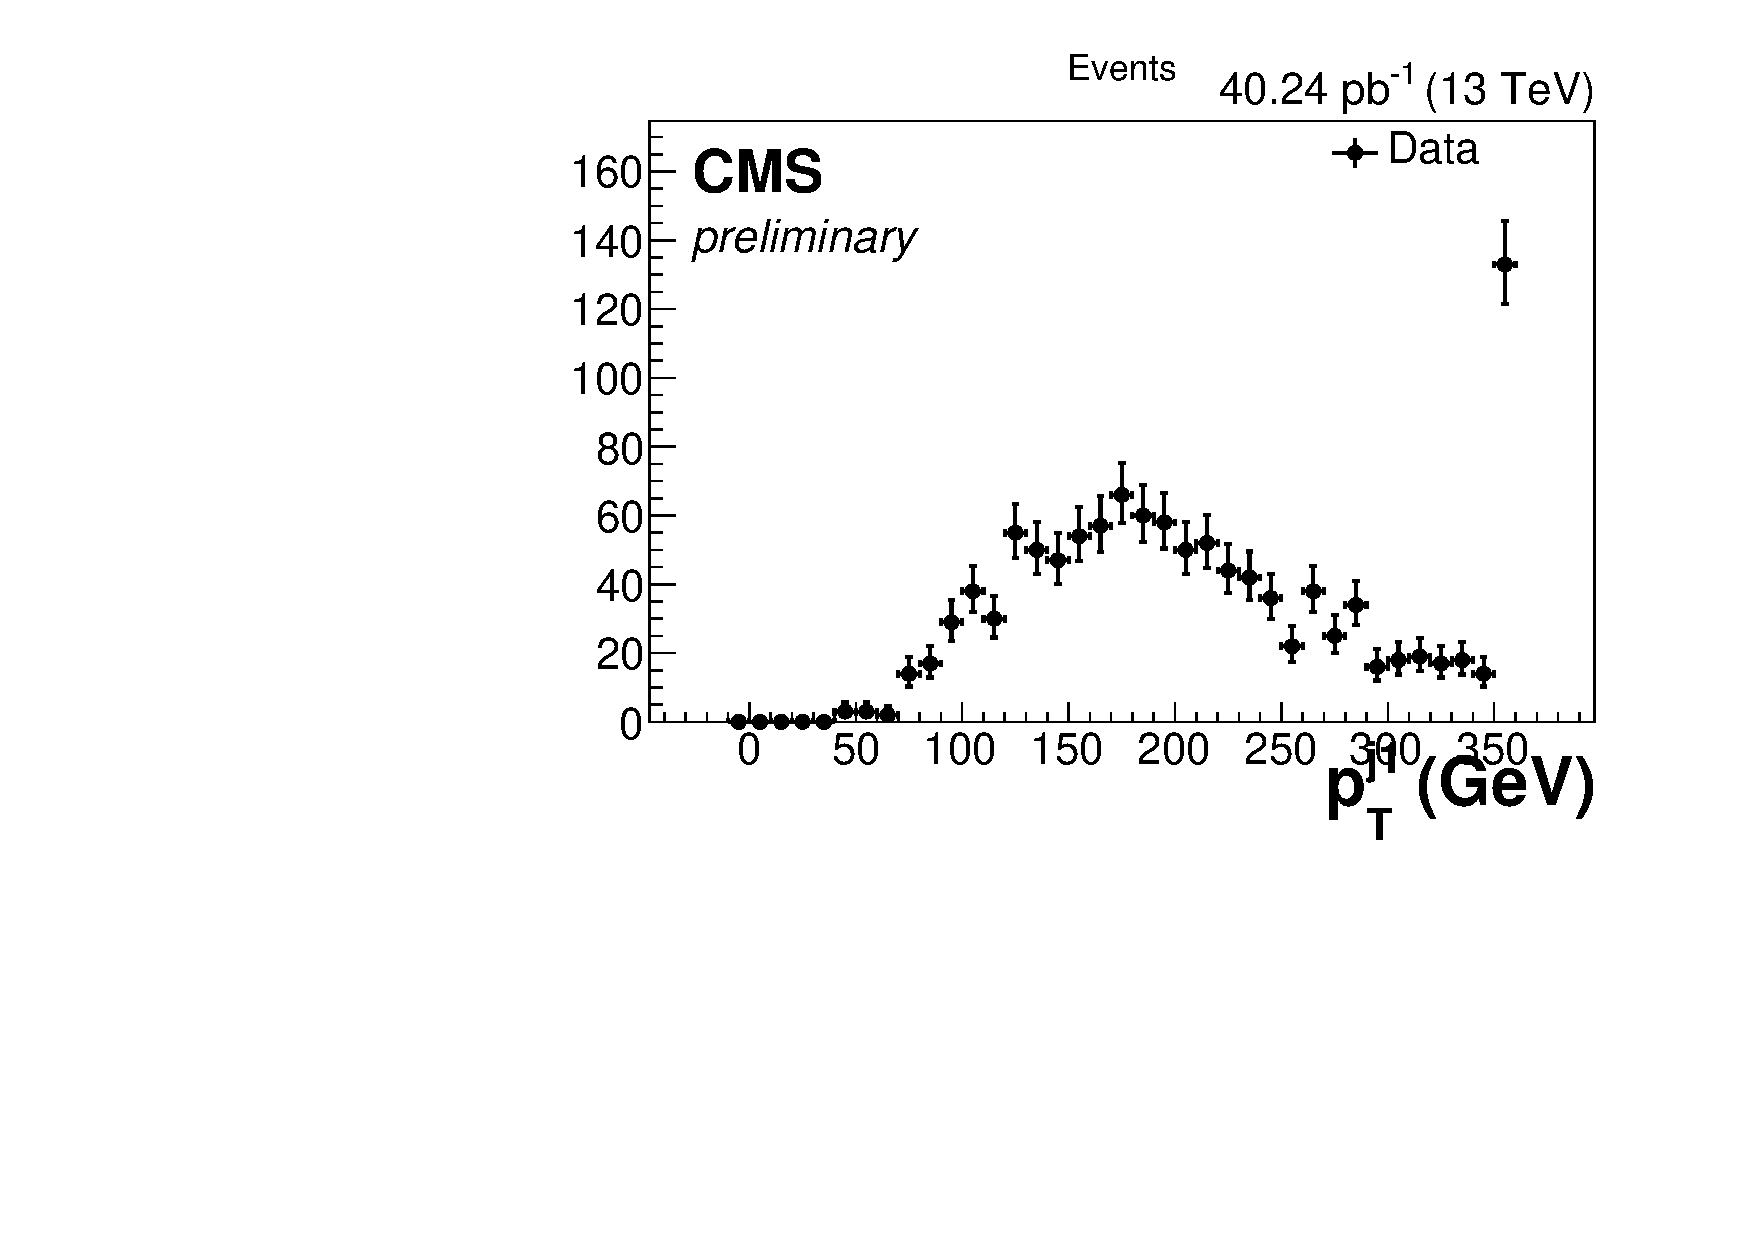
\includegraphics[width=.5\textwidth]{TalkPics/dataplots030815/output/nunu_jet1_pt.pdf}
  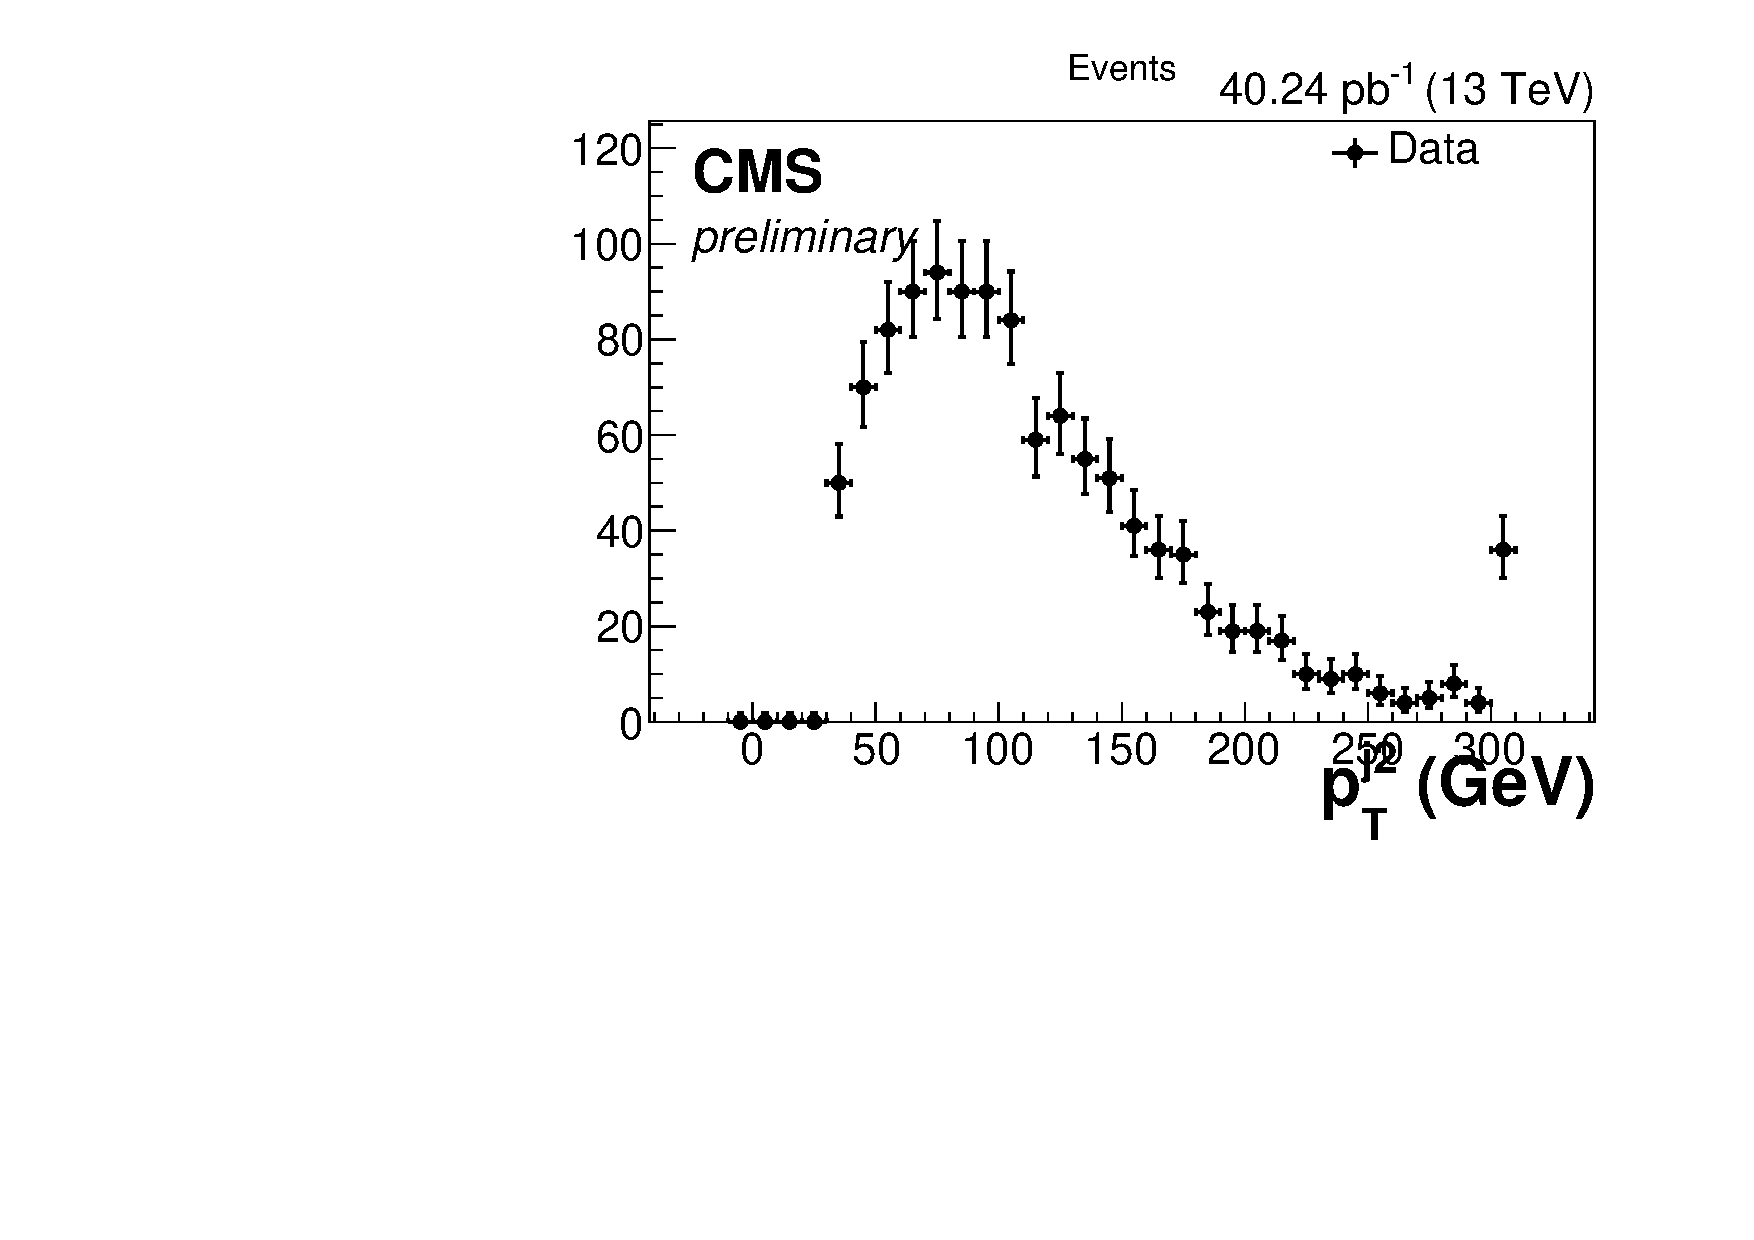
\includegraphics[width=.5\textwidth]{TalkPics/dataplots030815/output/nunu_jet2_pt.pdf}
\end{frame}

\begin{frame}
  \frametitle{Trigger variables: pass trigger}
  \begin{block}{}
    \begin{itemize}
    \item Start by requiring only HLT\_DiPFJet40\_DEta3p5\_MJJ600\_PFMETNoMu140\_v
    \end{itemize}
  \end{block}
  \centering
  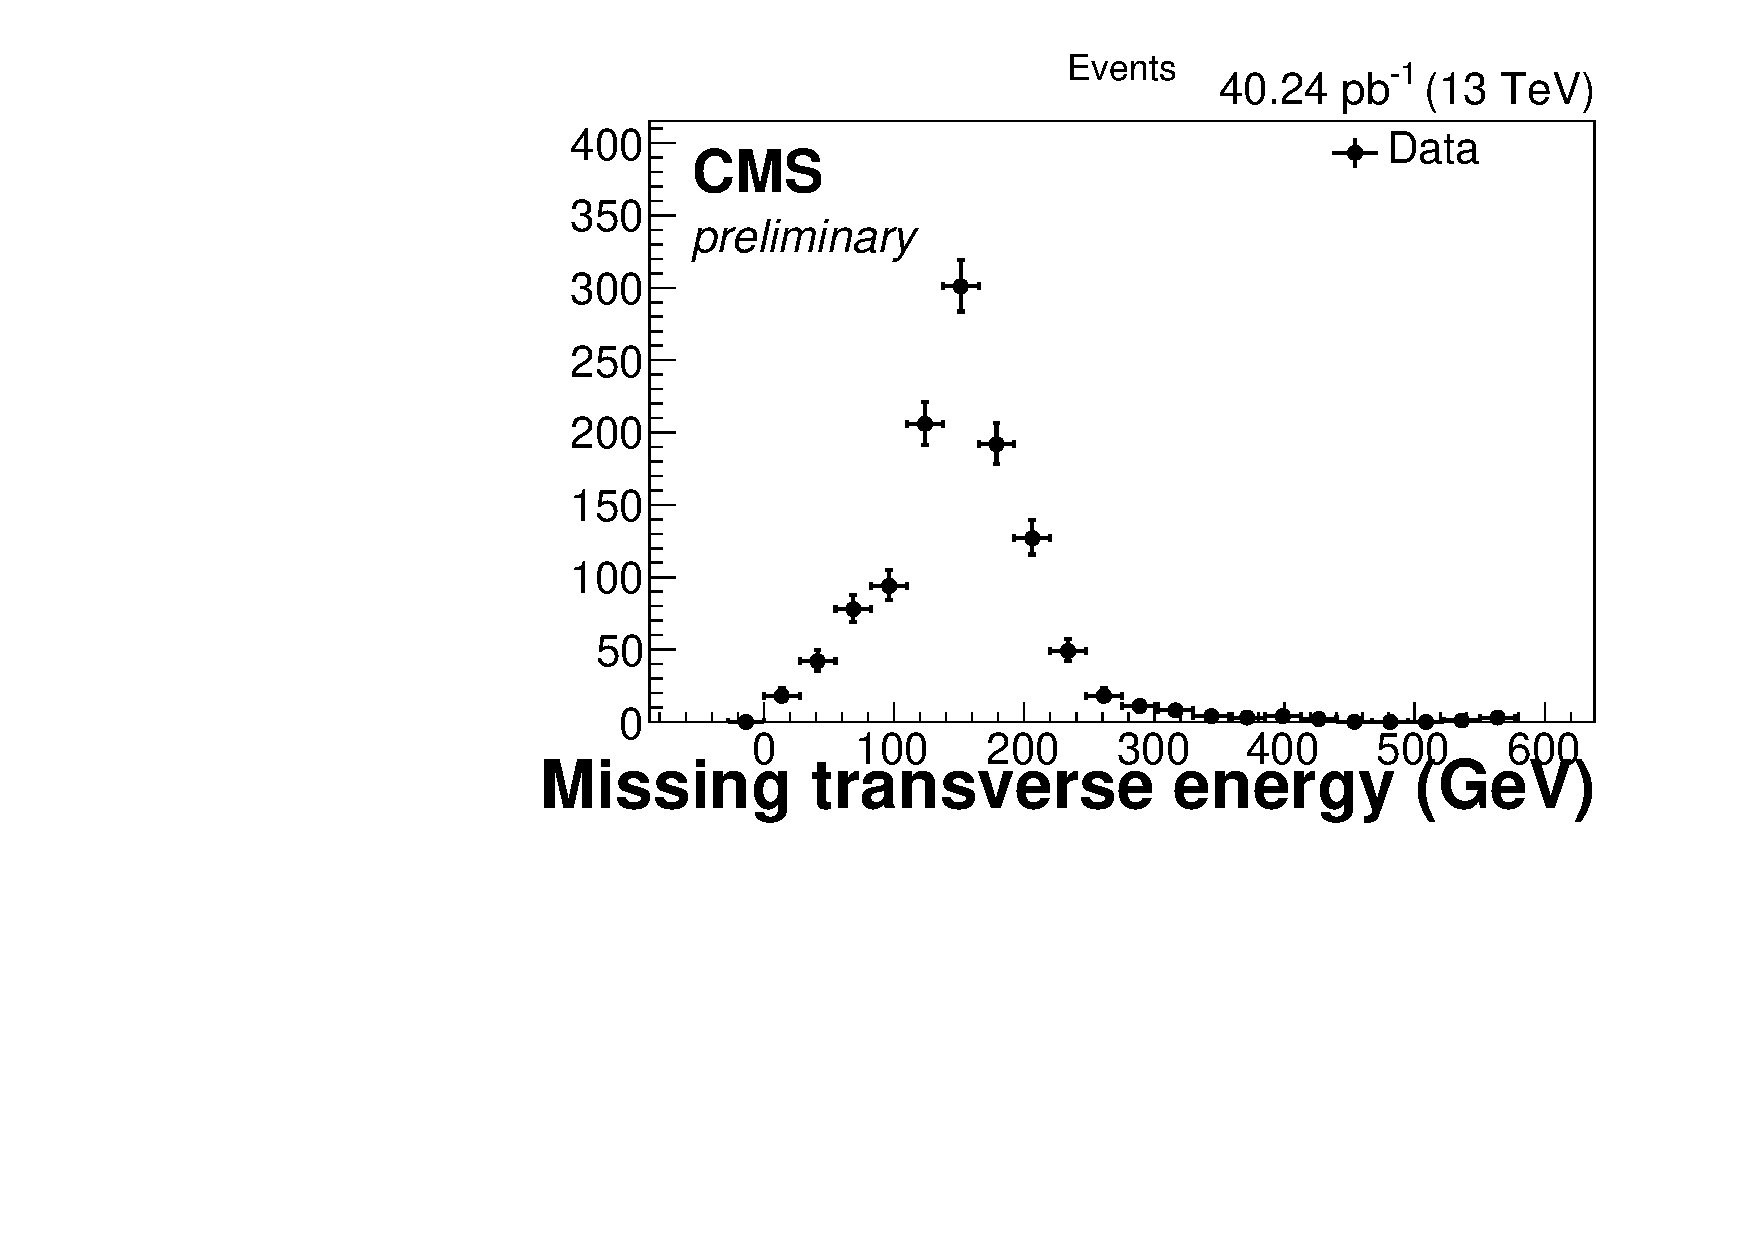
\includegraphics[width=.5\textwidth]{TalkPics/dataplots030815/output/nunu_metnomuons.pdf}
\end{frame}

\begin{frame}
  \frametitle{Trigger variables: tighten cuts}
  \begin{block}{}
    \begin{itemize}
    \item Check $\Delta\eta_{jj}$ and $M_{jj}$ for events with:
    \item[-] 2 jets $p_{T}>40$ GeV
    \end{itemize}
  \end{block}
  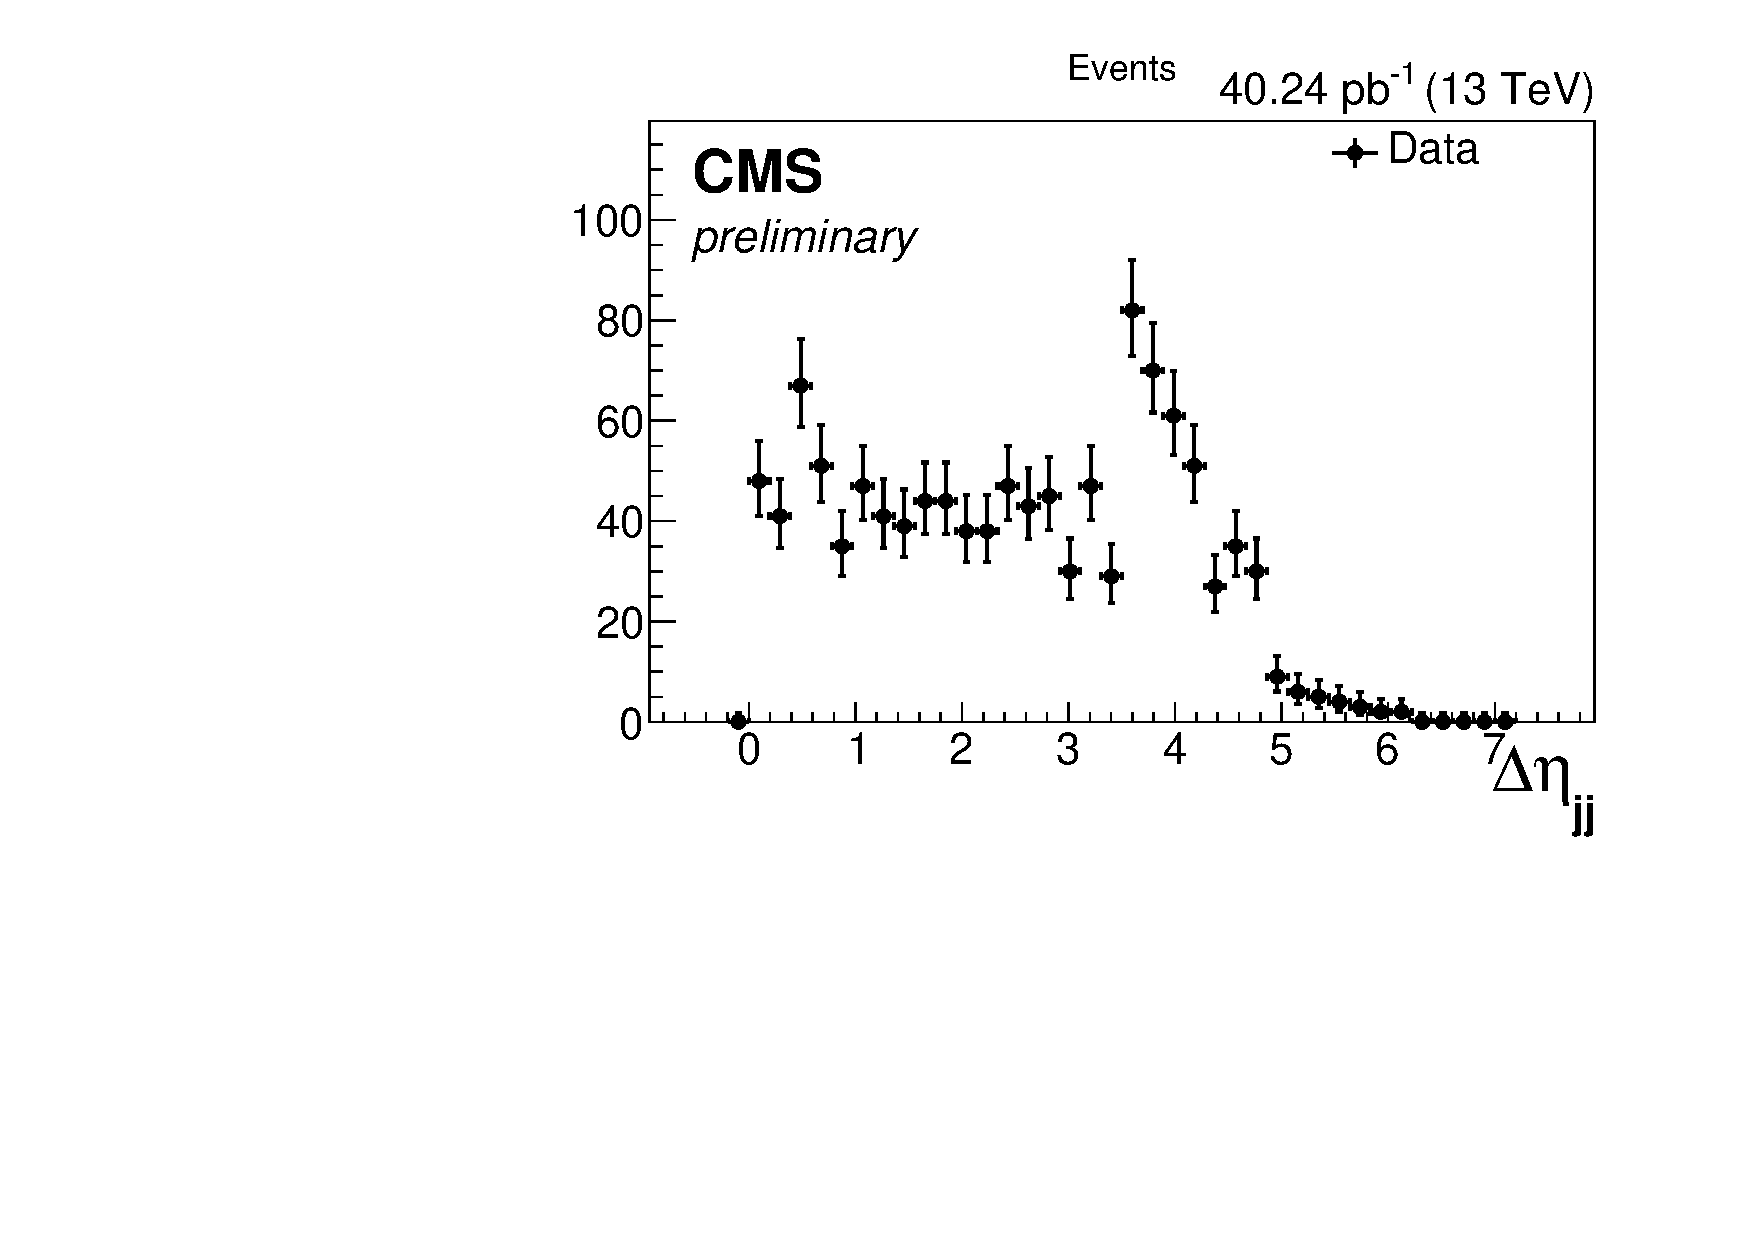
\includegraphics[width=.5\textwidth]{TalkPics/dataplots030815/output/nunu_jpt40_dijet_deta.pdf}
  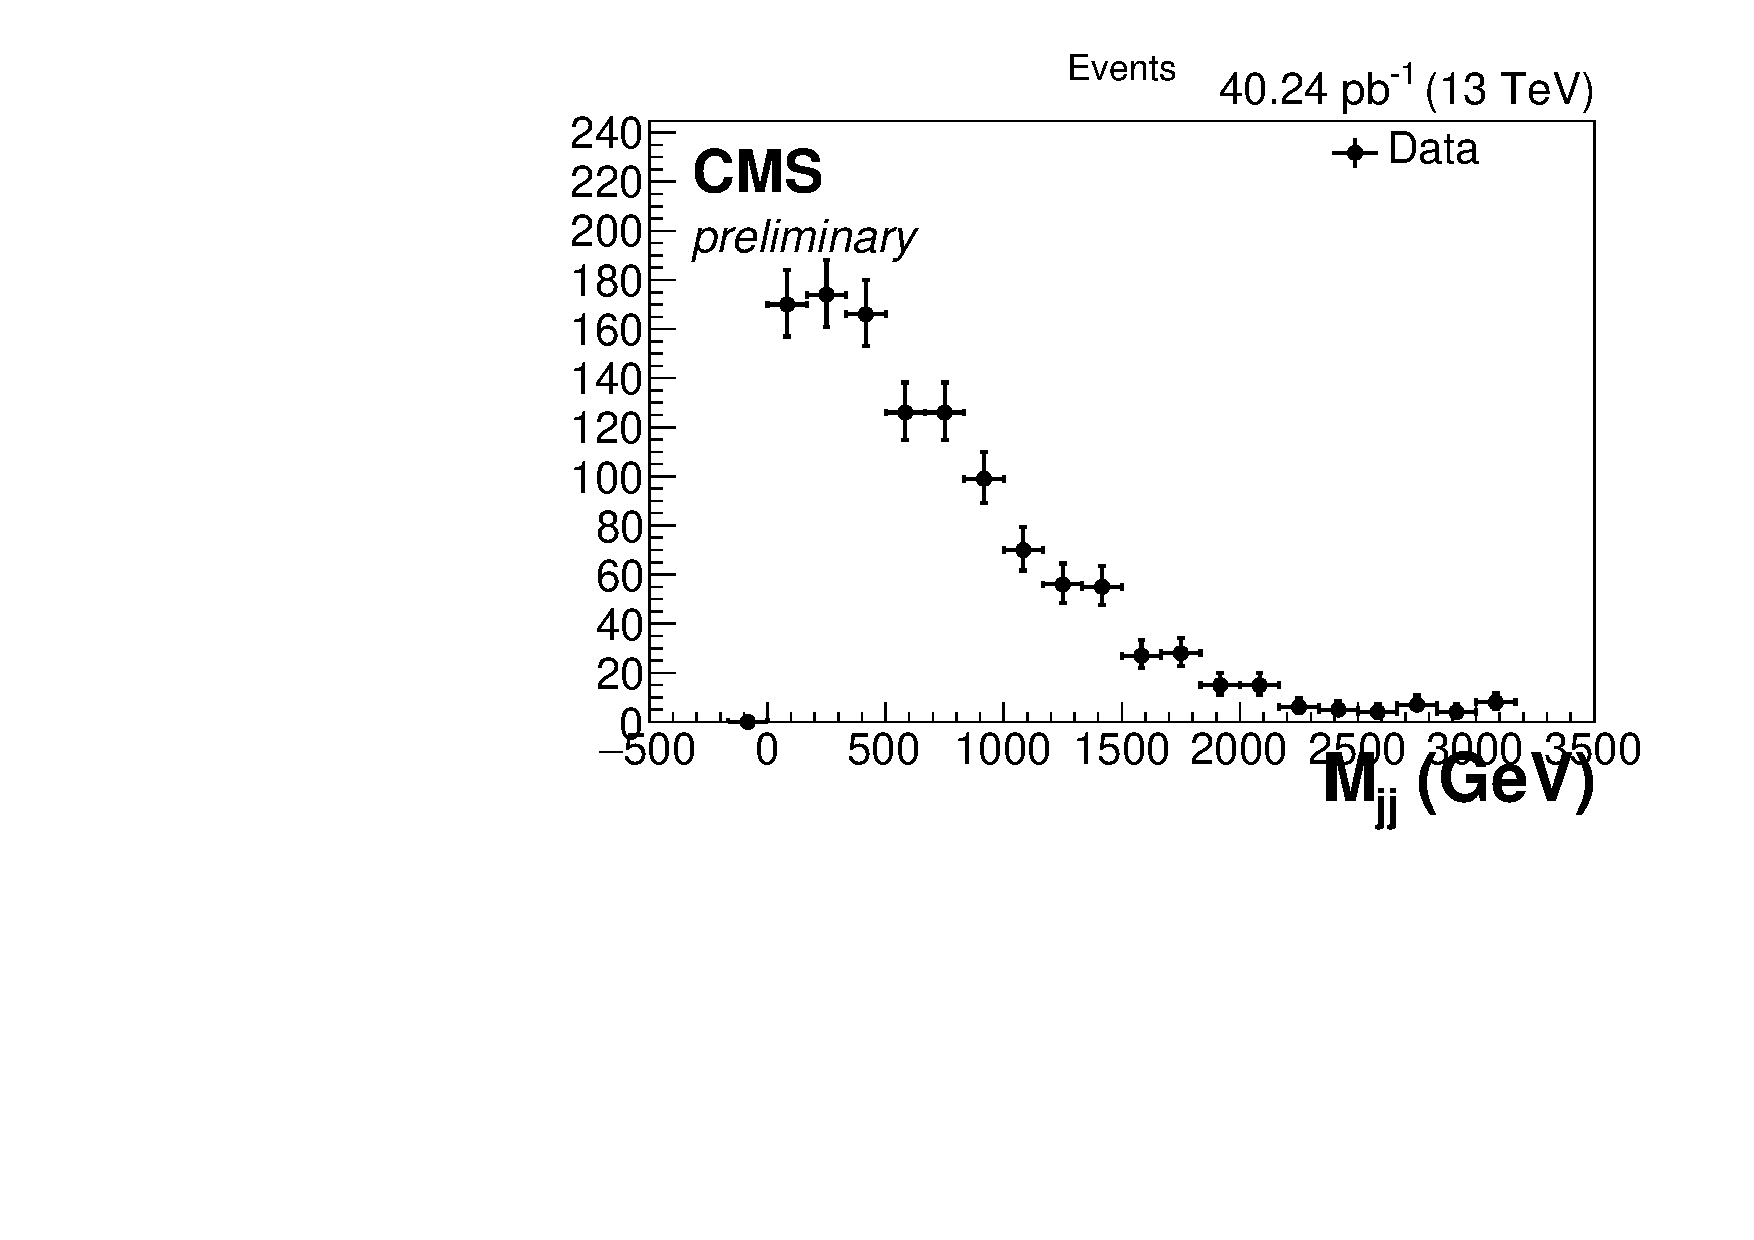
\includegraphics[width=.5\textwidth]{TalkPics/dataplots030815/output/nunu_jpt40_dijet_M.pdf}
  \begin{block}{}
    \begin{itemize}
    \item No difference
    \end{itemize}
  \end{block}
\end{frame}

\begin{frame}
  \frametitle{Trigger variables: tighten cuts}
  \begin{block}{}
    \begin{itemize}
    \item For $\Delta\eta_{jj}$ also require $M_{jj}>600$ GeV
    \item For $M_{jj}$ also require $\Delta\eta_{jj}>3.5$
    \end{itemize}
  \end{block}
  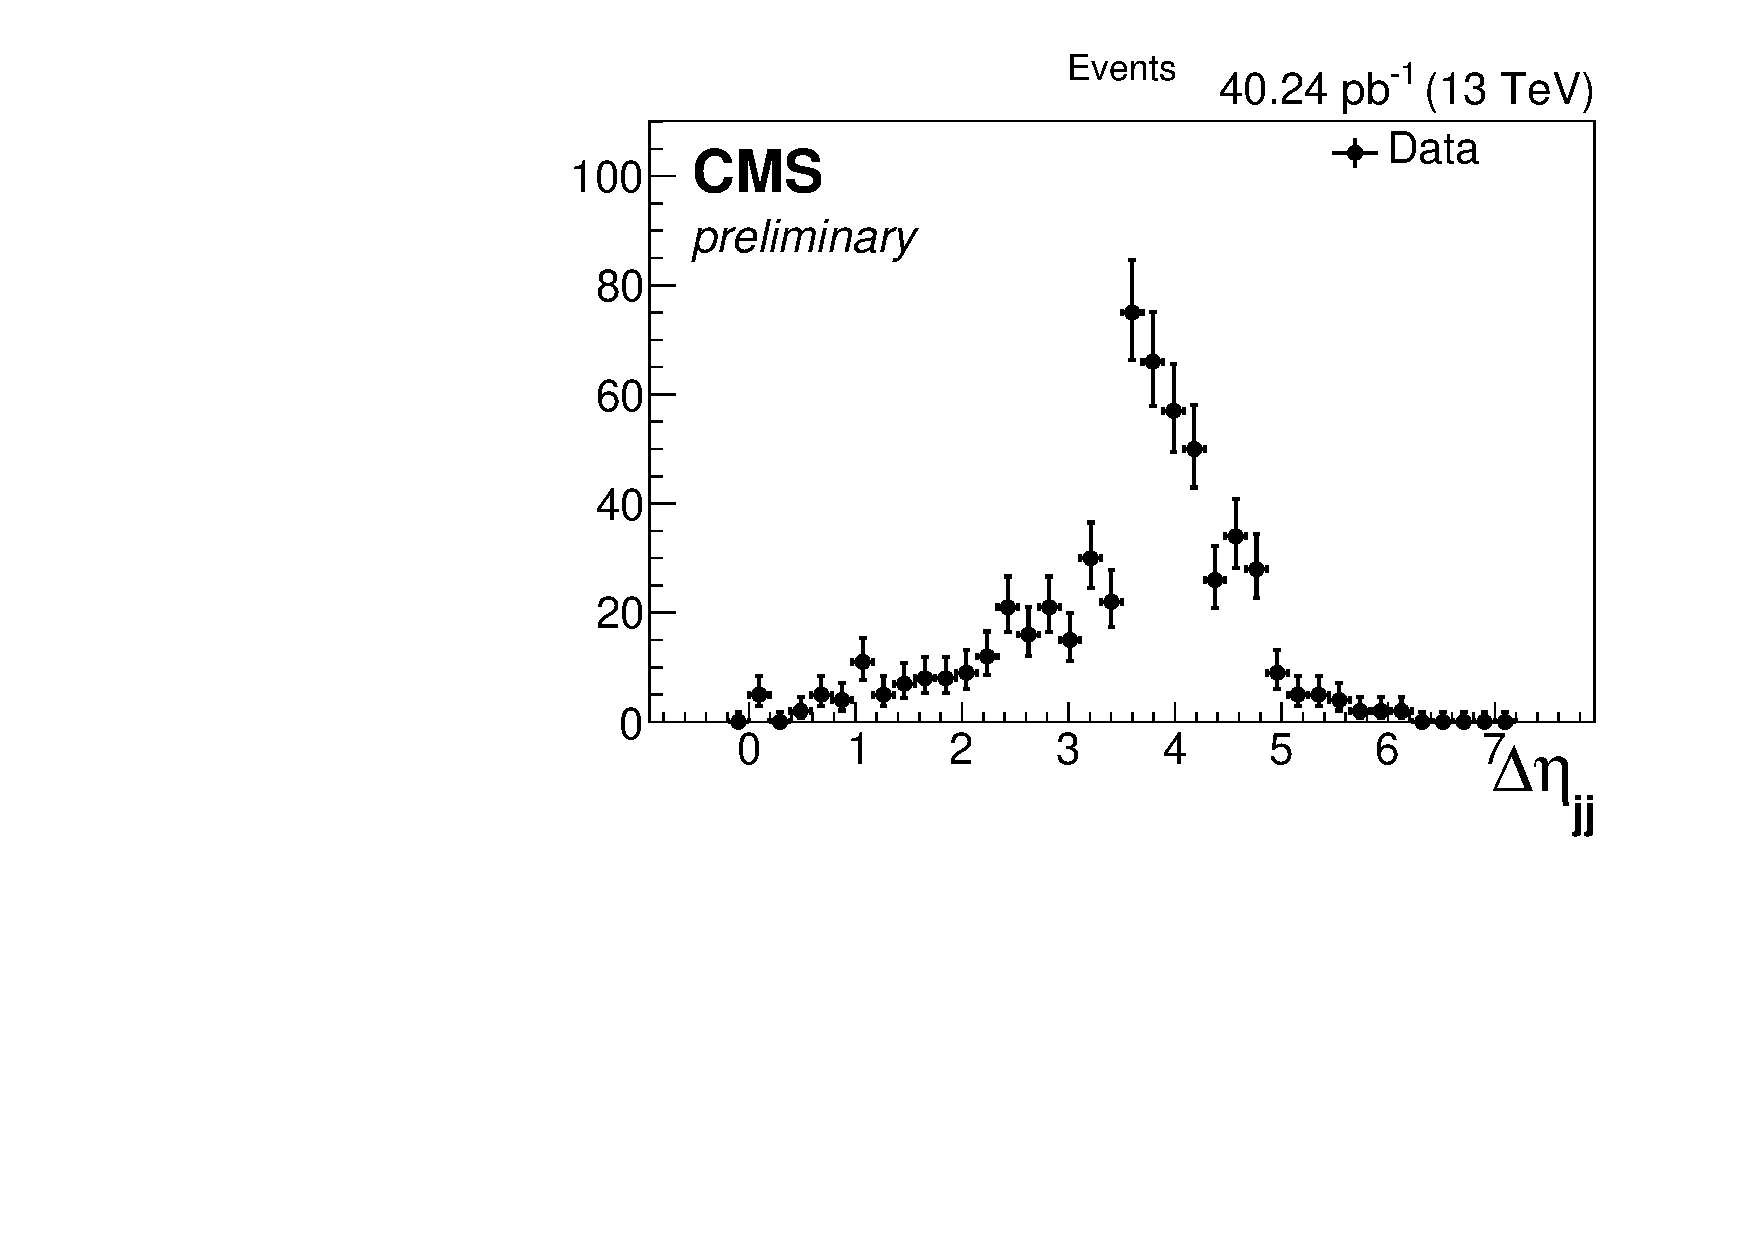
\includegraphics[width=.5\textwidth]{TalkPics/dataplots030815/output/nunu_jpt40dijetm600_dijet_deta.pdf}
  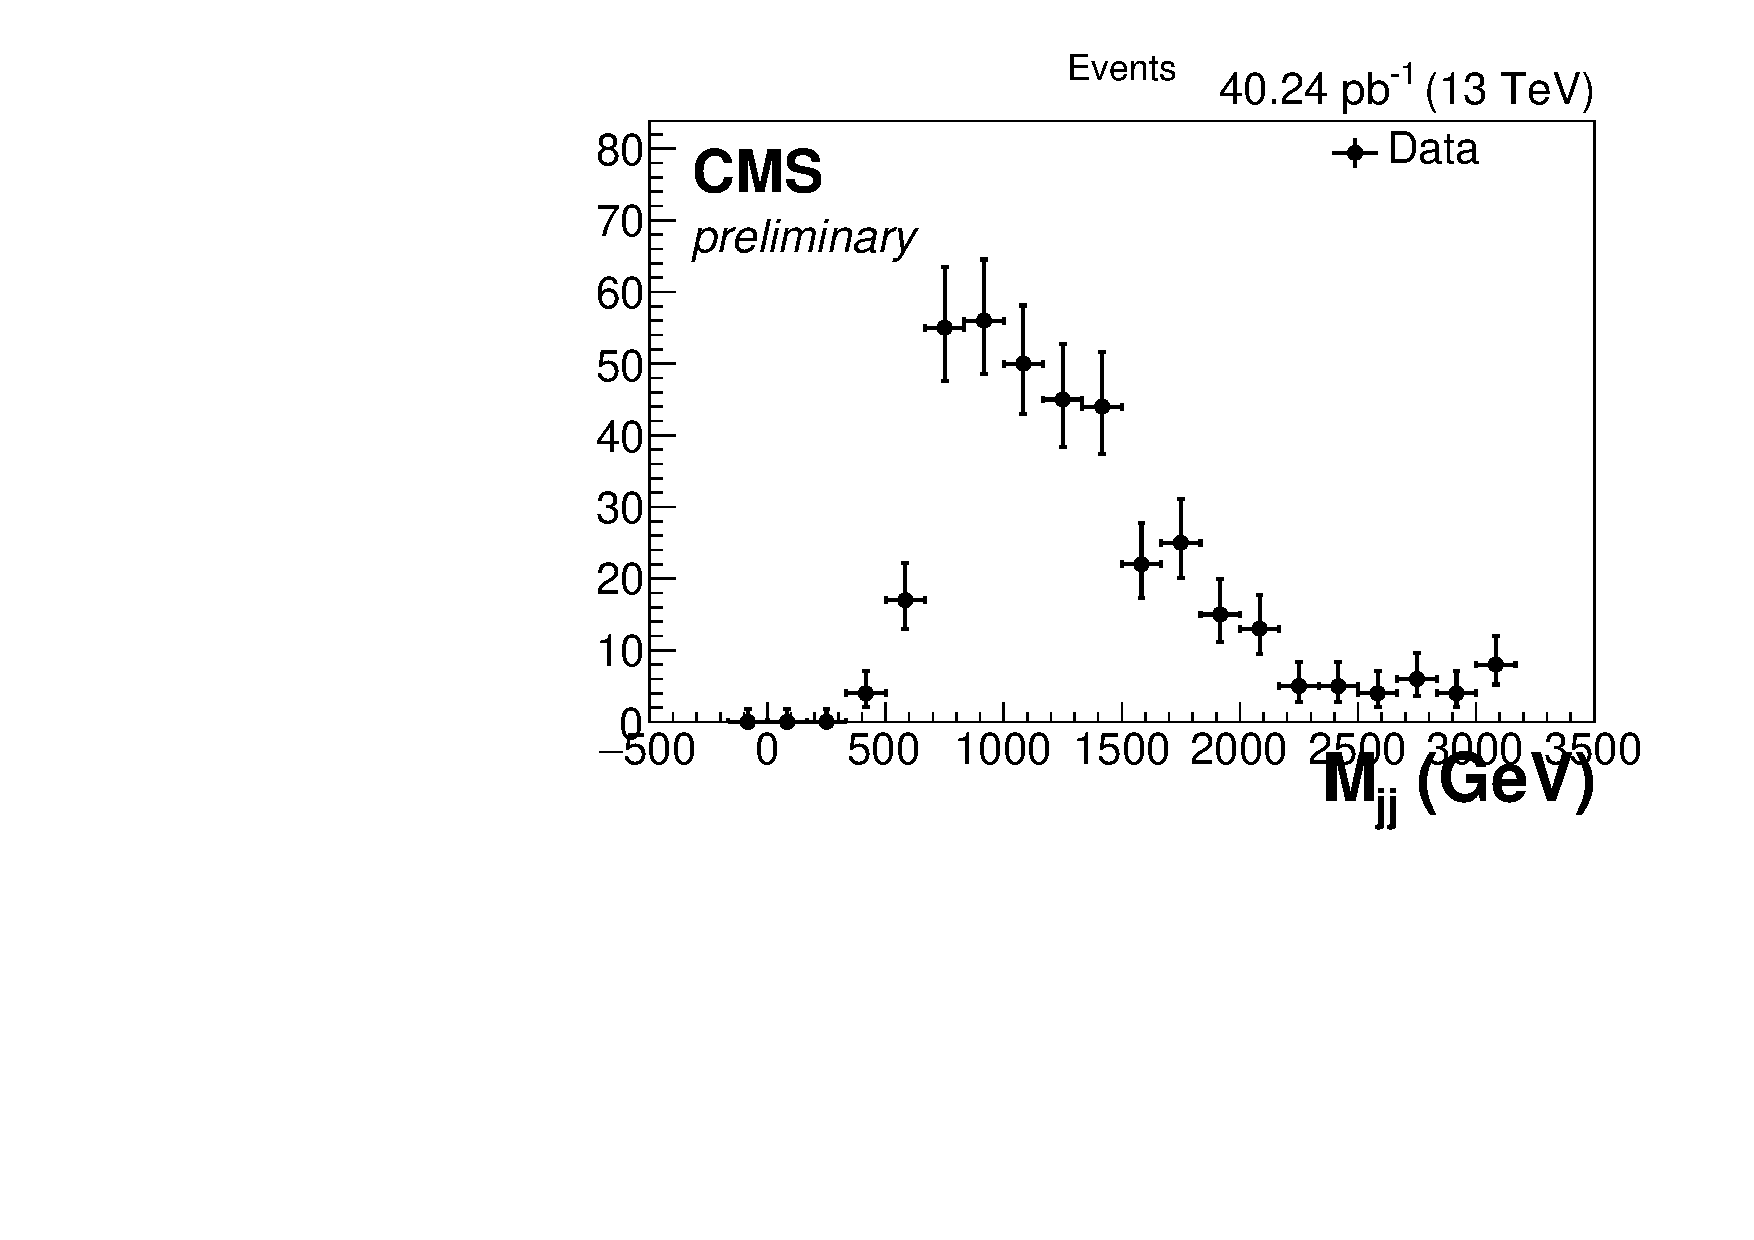
\includegraphics[width=.5\textwidth]{TalkPics/dataplots030815/output/nunu_jpt40deta35_dijet_M.pdf}
  \begin{block}{}
    \begin{itemize}
    \item Much better
    \end{itemize}
  \end{block}
\end{frame}


\begin{frame}
  \frametitle{Trigger variables: MET with tighter cuts}
  \begin{block}{}
    \begin{itemize}
    \item Require 2 jets $p_{T}>40$ GeV, $M_{jj}>600$ GeV, $\Delta\eta_{jj}>3.5$
    \end{itemize}
  \end{block}
  \centering
  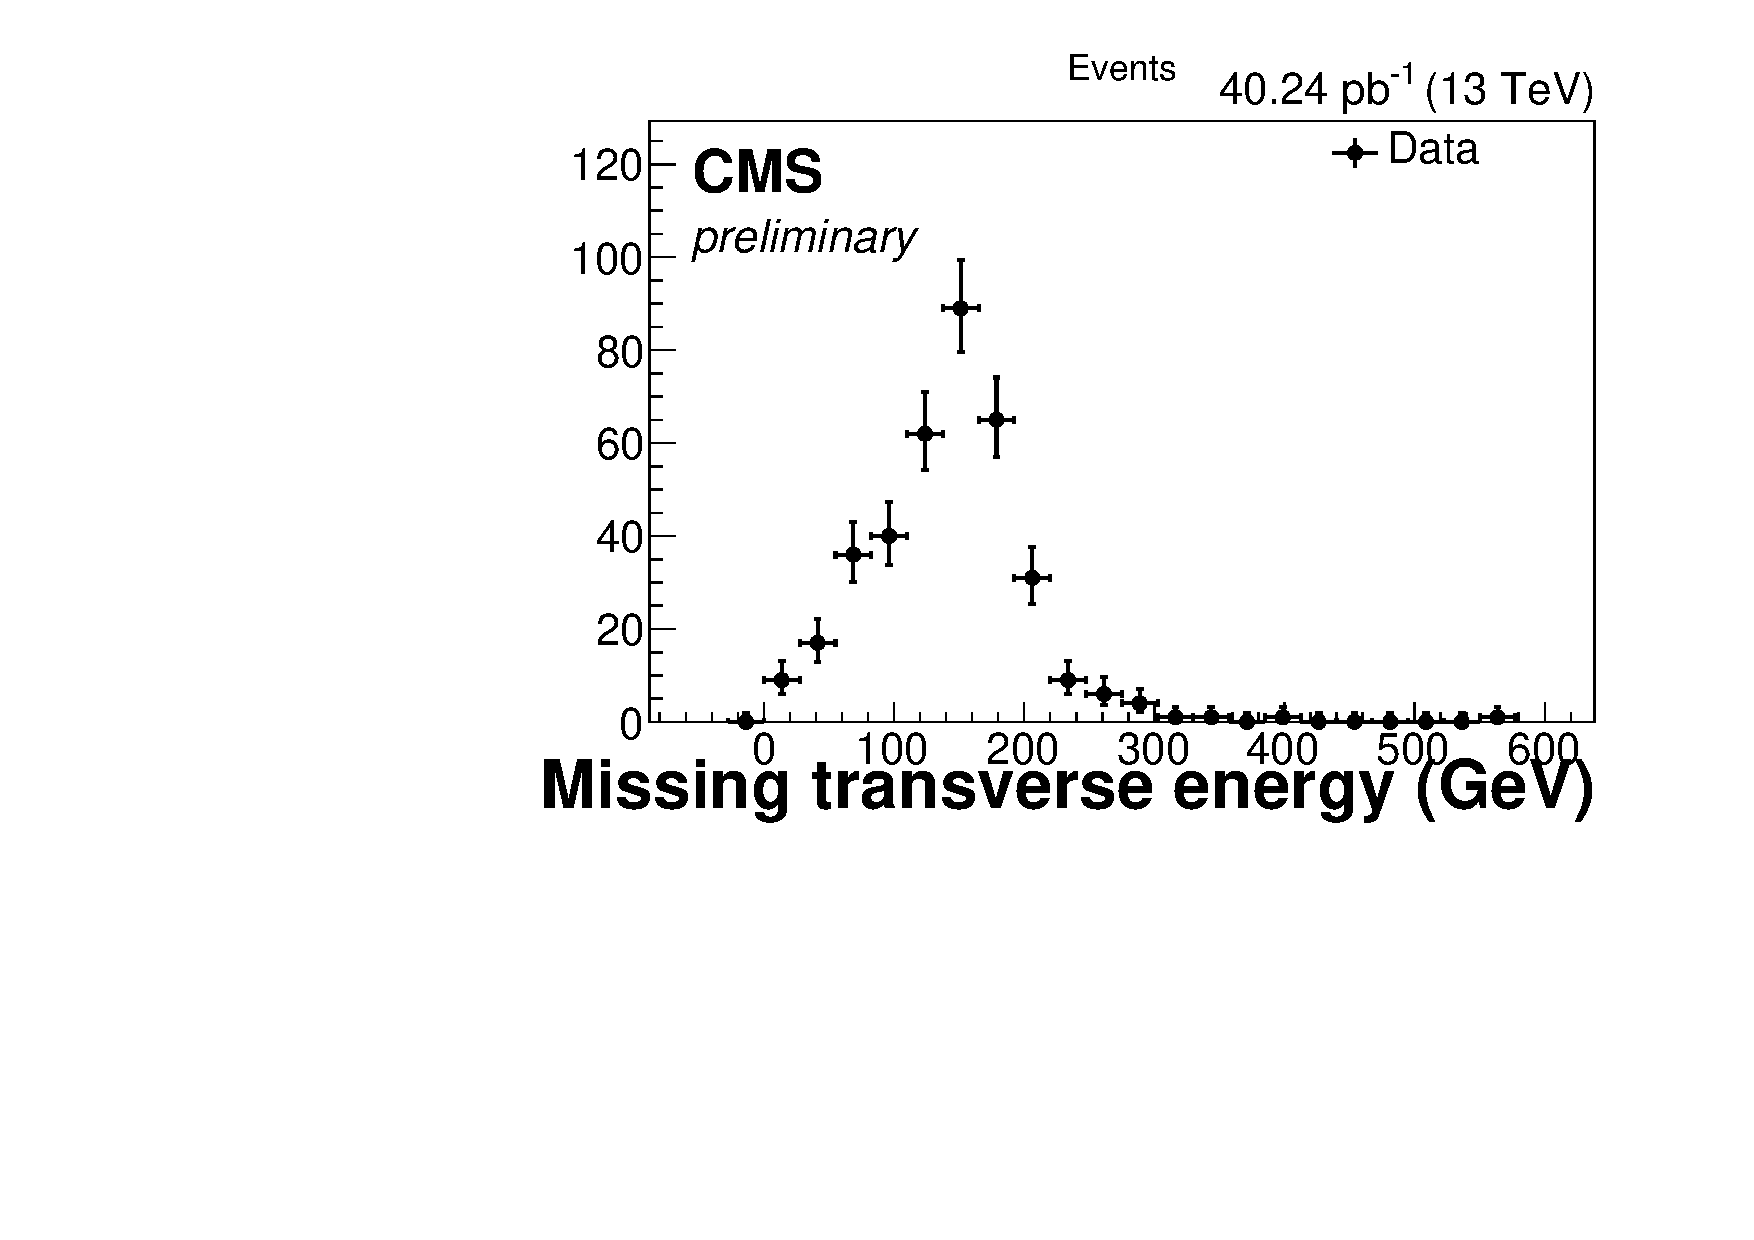
\includegraphics[width=.5\textwidth]{TalkPics/dataplots030815/output/nunu_jpt40dijetM600deta35_metnomuons.pdf}
\end{frame}

\begin{frame}
  \frametitle{Combination}
  \begin{block}{}
    \begin{itemize}
    \item Expected limit 30\%
    \item Preapproval in Higgs meeting next Tuesday
    \end{itemize}
  \end{block}
  \begin{columns}
    \column{.5\textwidth}
    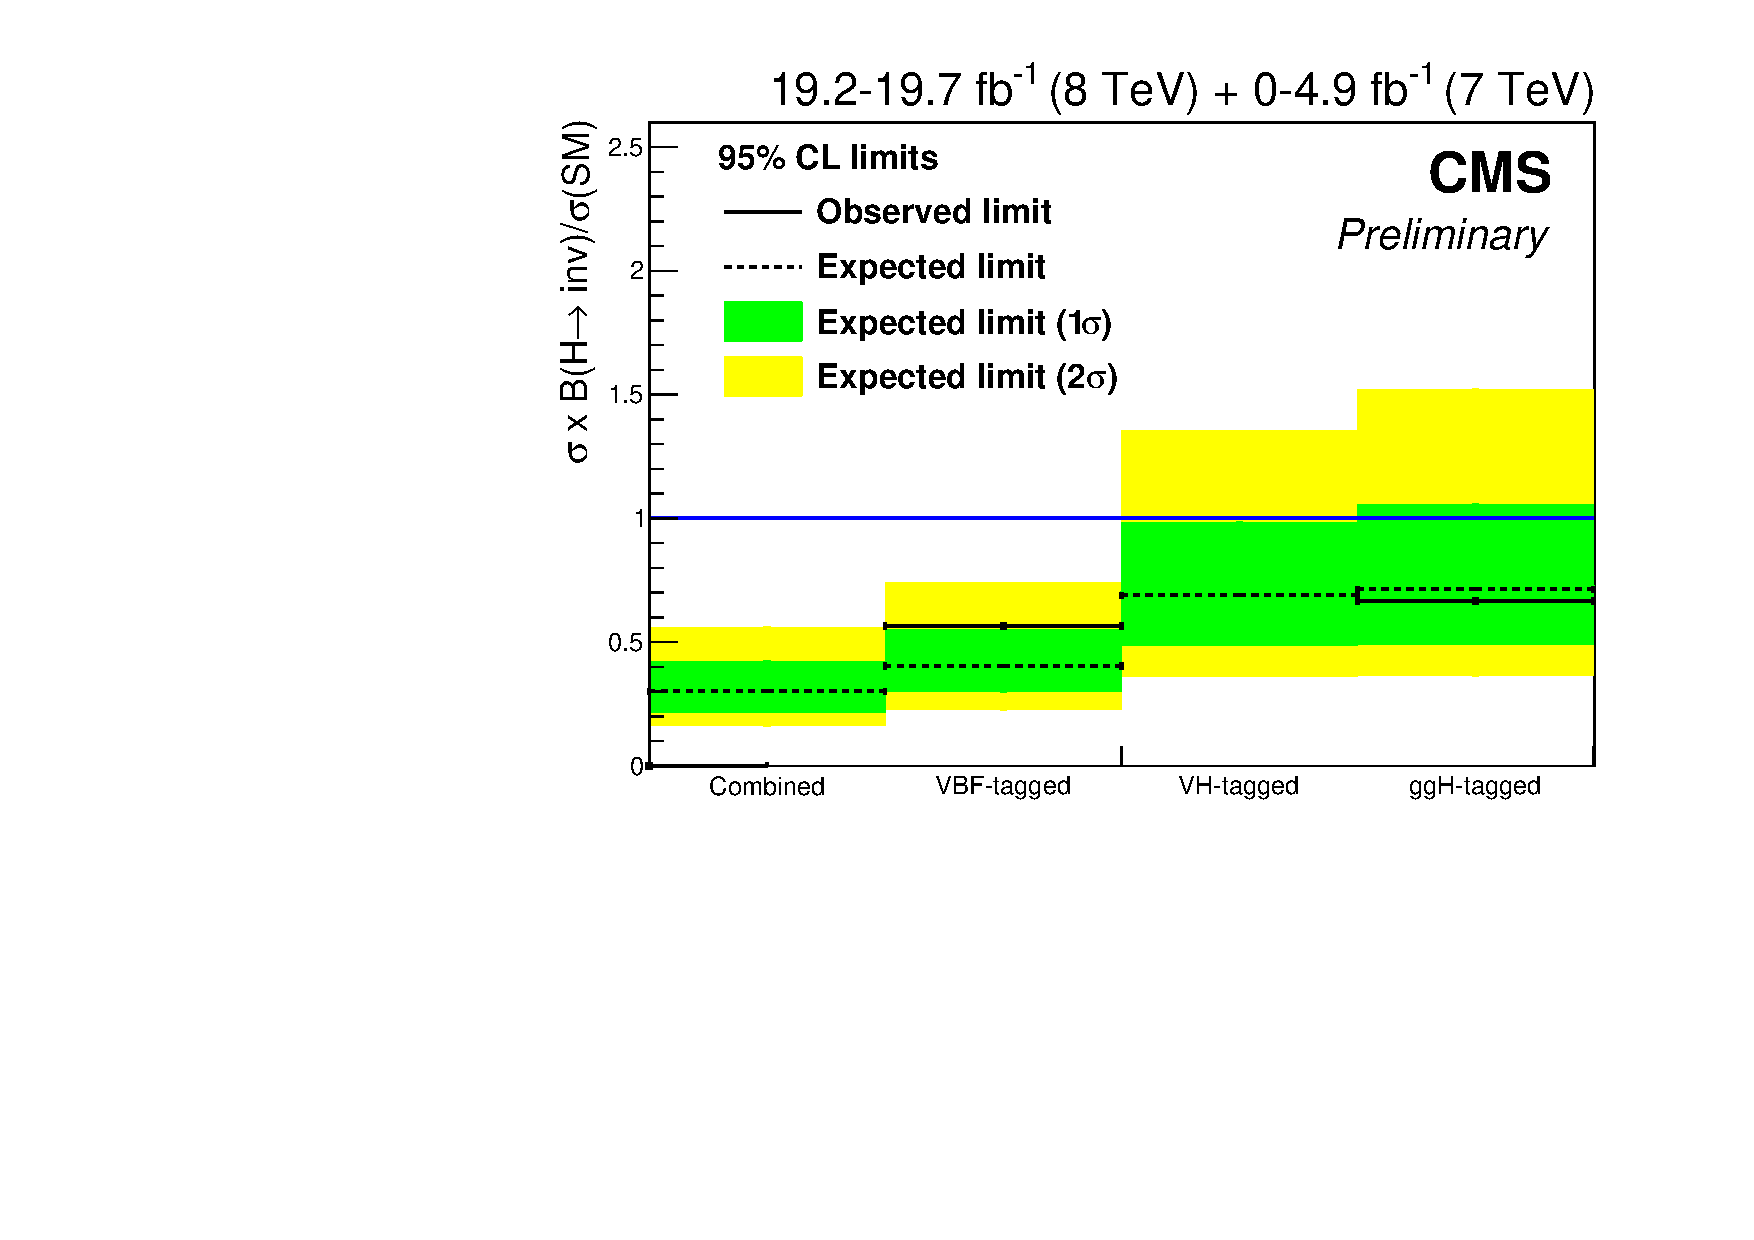
\includegraphics[width=\textwidth]{TalkPics/dataplotsandcomb040815/channellimit.pdf}
    \column{.5\textwidth}
    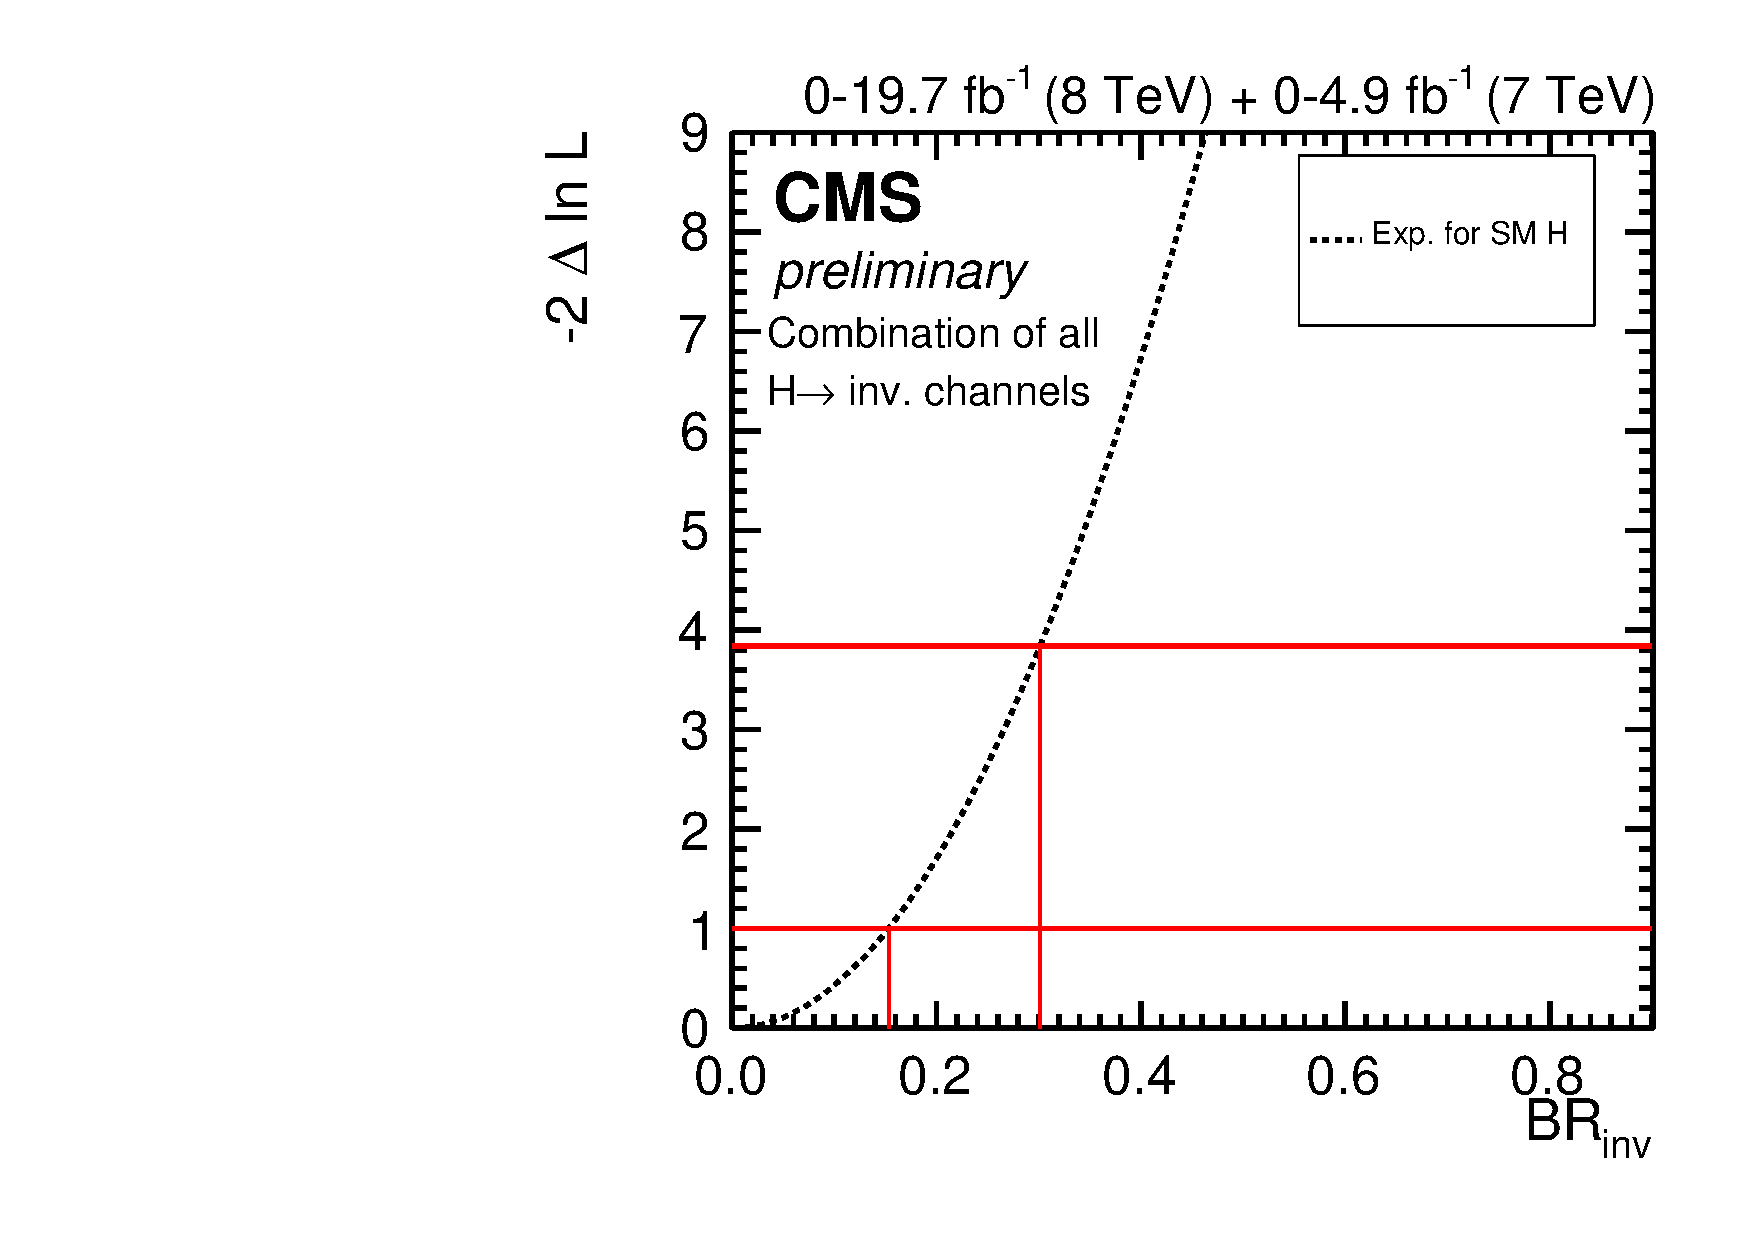
\includegraphics[width=\textwidth]{TalkPics/dataplotsandcomb040815/combscan.pdf}
  \end{columns}
  \begin{block}{}
    \begin{itemize}
    \item Much better
    \end{itemize}
  \end{block}
\end{frame}



\begin{frame}
  \label{lastframe}
  \begin{block}{Summary}
    \begin{itemize}
    \item Trigger variables look roughly as expected
    \item Next steps:
    \item[-] Turn on curves from single mu
    \item[-] Get MC expectations for comparison
    \item Combination progress:
    \item[-] First draft of PAS and updated Exo AN are in CADI
    \item[-] Preapproval next Tuesday
    \end{itemize}
  \end{block}
\end{frame}

\begin{frame}
  \frametitle{Backup}
\end{frame}

\end{fmffile}
\end{document}
